\documentclass[12pt]{article} 
\usepackage{longtable}
\usepackage{makecell}
\usepackage{float}
\usepackage{graphicx}
\usepackage{bm}
\usepackage{placeins}
\usepackage{booktabs}
\usepackage{gensymb}
\usepackage{subcaption}
\usepackage{amssymb}
\usepackage{indentfirst}
\usepackage{threeparttable} 
\usepackage{multirow}
\usepackage{tabularx}
\usepackage{aligned-overset}
\usepackage[slantfont,boldfont]{xeCJK}
\usepackage{fontspec}
\renewcommand{\arraystretch}{1.5}
% \usepackage[paperwidth=21cm,paperheight=29.7cm]{geometry}
\usepackage[a4paper,margin=2cm]{geometry}
\usepackage{siunitx}

\sisetup{
  table-number-alignment = center,
  table-format = 1.3,
  table-space-text-pre  = {},
  table-space-text-post = {},
  table-sign-mantissa = false,
  table-align-text-pre = false,
  table-align-text-post = false
}

\setlength{\LTpre}{0pt}
\setlength{\LTpost}{0pt}
\setCJKmainfont{SimSun}
\setmainfont{SimSun}
\setsansfont{SimSun}
% 设置正文字体为四号（12pt）
% \renewcommand{\CJKmainfont}{SimSun}
\renewcommand{\CJKfamilydefault}{\CJKrmdefault}
\renewcommand{\normalsize}{\fontsize{12pt}{18pt}\selectfont}
\normalsize

\title{霍尔效应实验报告}
\author{2411545 邱凯锐}
\date{2025.1.4}

\begin{document}
\maketitle
\section{实验原理}
\subsection{霍尔效应基本机制}
当电流 $I_H$ 通过霍尔元件（假设为P型半导体），且该元件置于垂直于电流方向的磁场 $B$
中时，载流子（空穴）会受到洛伦兹力的作用。
\begin{equation}
    \vec F_B=q(\vec v\times \vec B)
\end{equation}
其中 $q$ 为电荷量，$\vec v$ 为漂移速度。

洛伦兹力使载流子发生横向偏转，并在元件的侧面（边界）积累，从而产生一个横向电
场 $E$。当电场力 $F_E=q E$ 与洛伦兹力 $F_B$ 达到平衡，载流子不再偏转，此时建立的电势差即
为霍尔电势差，记为 $U_H$ 。
\begin{equation}
    q(\vec v\times \vec B)=q\vec E \Rightarrow E=vB
\end{equation}

\subsection{霍尔电压与灵敏度公式推导}
设霍尔元件宽度为 $\omega$ ，厚度为 $d$ ，载流子浓度为 $p$ 。通过样品的电流 $I_H=pq\omega dv$，则载流子速度 $v=\dfrac{I_H}{pq\omega d}$
于是
\begin{equation}
    U_H=E\omega=vB\omega =\frac{I_H}{pq\omega d}B\omega =\frac 1{pqd}I_HB
\end{equation}
令 $R_H=\dfrac{1}{pq}$ 为霍尔系数，$K_H=\dfrac{R_H}{d}=\dfrac{1}{pqd}$ 为霍尔元件灵敏度，单位为 $\mathrm{mV/(mA\cdot T)}$，则
\begin{equation}
    U_H=\left(\frac{R_H}{d}\right)I_HB=I_H K_HB
\end{equation}

\subsection{消除霍尔元件副效应}
在实际测量中，霍尔电极两端的电压不仅包含霍尔电压 $U_H$ ，还包含多种伴随产生的热磁副效应和不等位电势差。
\begin{itemize}
    \item 不等位电势差 $U_0$：由于霍尔电极不在同一等势面上（欧姆接触点不对称）产生。方向随 $I_H$ 改变。
    \item 埃廷斯豪森效应 $U_E$：纵向电流与磁场作用导致横向温差，产生温差电动势。方向随 $I_H$ 和 $B$ 改变。
    \item 能斯特效应 $U_N$：纵向热流与磁场作用产生横向温差，进而产生温差电动势，只与 $B$ 和热流有关。
    \item 里吉-勒迪克效应 $U_R$：纵向热流与磁场作用产生横向温差，进而产生温差电动势。只与 $B$ 和热流有关。
\end{itemize}

为了消除上述误差，实验采用改变电流 $I_H$ 方向和改变磁场 $B$ 方向的组合测量法。记录电压数据：
\begin{itemize}
    \item $I_H$ 正，$B$ 正：$U_1=U_H+U_0+U_E+U_N+U_R$
    \item $I_H$ 负，$B$ 正：$U_2=-U_H-U_0-U_E+U_N+U_R$
    \item $I_H$ 负，$B$ 负：$U_3=U_H-U_0+U_E-U_N-U_R$
    \item $I_H$ 正，$B$ 负：$U_4=-U_H+U_0-U_E-U_N-U_R$
\end{itemize}
由于在实际中 $U_H\gg U_E$，可以得到
\begin{equation}
    U_H=\frac 14(U_1-U_2+U_3-U_4)
\end{equation}

\section{实验仪器}
\subsection{新型螺线管磁场测定仪}
虽然从理论上讲霍尔元件在无磁场作用（即$B=0$）时，$U_H=0$，但是实际情况用数字
电压表测时并不为零，这是由于半导体材料结晶不均匀及各电极不对称等引起附加电势差，
该电势差 $U_0$ 称为剩余电压。

随着科技的发展，新的集成化(IC)元件不断被研制成功。本实验采用 SS95A 型集成霍
尔传感器（结构示意图如图所示）是一种高灵敏度集成霍尔传感器，它由霍尔元件、放大器
和薄膜电阻剩余电压补偿组成。测量时输出信号大，并且剩余电压的影响已被消除。
对SS95A型集成霍尔传感器，它由三根引线，分别是：“$V_+$”、“$V_-$”、“$V_{out}$”。其中“
$V_+$”和“$V_-$”构成“电流输入端”，“$V_{out}$”和“$V_-$”构成“电压输出端”。由于SS95A
型集成霍尔传感器，它的工作电流已设定，被称为标准工作电流，使用传感器时，必须使工
作电流处在该标准状态。在实验时，只要在磁感应强度为零（零磁场）条件下，调节“$V_+$”、“$V_-$”所接的电源电压（装置上有一调节旋钮可供调节），使输出电压为2.500 V（在
数字电压表上显示），则传感器就可处在标准工作状态之下。

当螺线管内有磁场且集成霍尔传感器在标准工作电流时，与式相似，由式可得：
\begin{equation}
    B=\frac{(U-2.500)}{K}=\frac{U'}{K}
\end{equation}
式中 $U$ 为集成霍尔传感器的输出电压，$K$ 为该传感器的灵敏度，$U'$ 经用 2.500 V 外接电压
补偿以后，用数字电压表测出的传感器输出值（仪器用 mV 档读数）。
\begin{figure}[H]
    \centering
    
\includegraphics[width=0.6\textwidth]{fig1.png}
    \caption{集成霍尔元件内部结构图}
\end{figure}

FD-ICH-II 新型螺线管磁场测定仪由集成霍尔传感器探测棒、螺线管、直流稳压电源；数字电压表组成。
实验电源分三个部分，面板左面为数字式直流稳流源，用精密多圈电位器调节输出电流的大小，调节精度 $1\text{mA}$，
电流大小由三位半数字电流表显示；面板右边为四位半电压表，黑色拨动开关切换量程 $0—19.999\text{V}$ 和 $0—1999.9\text{mV}$。
面板中间为直流稳压电源,对应输出接线柱上方是调节输出电压电位器(顺时针调节电压增加)。仪器连线图如 Figure 2 所示。
\begin{figure}[H]
    \centering
    
\includegraphics[width=0.6\textwidth]{fig2.png}
    \caption{螺线管测量磁场仪器}
\end{figure}

\subsection{霍尔效应试验仪}
霍尔效应实验仪由可调直流稳压电源($0\text{—}500\text{mA}$)、直流稳流电源($0\text{—}5\text{mA}$)、直流数字电压表，数字式特斯拉计、
直流电阻(取样电阻)电磁铁、霍尔元件(砷化镓霍尔元件)、双刀双向开关、导线等。实验电路如 Figure 3 所示。
\begin{figure}[H]
    \centering
    
\includegraphics[width=0.6\textwidth]{fig3.png}
    \caption{霍尔效应试验仪}
\end{figure}

\section{实验内容}
\subsection{新型螺线管磁场测定仪}
(1)实验接线如 Figure 2 所示。左面数字直流稳流源的“励磁恒流输出”端接电流换向开关，然后接螺线管的线圈接线柱。
右面稳压电源 $4.8\text{V}—5.2\text{V}$ 的输出接线柱(红)接霍尔元件的 $V_+$ (即引脚2—红色导线)，直流稳压电源的 $\bot$ (黑)接线柱接霍尔元件的 $V_-$ (即引脚3—黑色导线)，
霍尔元件的 $V_{out}$（引脚1—黄色导线）接右边电压表‘电压输入’的 $+$ (红)接线柱。电压表切换到V档(即拨动开关向上拨)。

(2)检查接线无误后接通电源，断开电流换向开关K2（即K2处于中间位置时），使得集成霍尔传感器处于零磁场条件下。
集成霍尔传感器放在螺线管的中间位置($X=16.0\,\text{cm}$ 处)，调节中间直流电源 $4.8\text{V}—5.2\text{V}$ 的输出旋钮，使右边数字电压表显示 $2.500\text{V}$，
这时集成霍尔元件便达到了标准化工作状态，即集成霍尔传感器通过电流达到规定的数值，且剩余电压恰好达到补偿，$U_0=0\,\text{V}$。

(3)仍断开开关$\text{K}_2$，在保持“$V_+$”和“$V_-$”电压不变的情况下，把开关$\text{K}_1$指向2，调节 $2.4\text{V}—2.6\text{V}$
电源输出电压，使数字电压表指示值为0(这时应将数字电压表量程拨动开关指向$\text{mV}$档)，也就是用一外接$2.500\text{V}$的电位差与传感器输出$2.500\text{V}$电位差进行补偿，这样就可直接用数字电压表读出集成霍尔传感器电势差的值$U'$。

(4)测定霍尔传感器的灵敏度$K$

(i) 改变输入螺线管的直流电流$I_{m}$，将传感器处于螺线管的中央位置(即$X=16.0\text{cm}$)，测量$U'—I_{m}$关系，记录10组数据，$I_{m}$范围在$0—500\text{mA}$，可每隔$50\text{mA}$测一次。做$U'—I_{m}$关系曲线。

\begin{table}[H]
    \centering
    \caption{测量霍尔电势差与通电螺线管电流 $I_m$ 的关系}
    \begin{tabular}{cccccccccccc}
        \hline\hline
        $I_m/\mathrm{mA}$ & 0    & 50   & 100  & 150  & 200  & 250   & 300   & 350   & 400   & 450   & 500   \\
        \hline
        $U/\mathrm{mV}$    & -2.6 & 19.7 & 42.9 & 65.2 & 88.4 & 110.9 & 133.8 & 156.5 & 179.2 & 202.1 & 225.1\\
        \hline\hline
    \end{tabular}
\end{table}

(ii)用最小二乘法求出$U' - I_{m}$直线的斜率$K' = \dfrac{\Delta U'}{\Delta I_{m}}$和相关系数$r$。

\begin{figure}[H]
    \centering
    
\includegraphics[width=0.8\textwidth]{Figure_1.png}
    \caption{}
\end{figure}

直线斜率 $K'=0.4555\ \mathrm{mV/mA}$，相关系数 $r=0.999997$。

(iii)对于无限长直螺线管磁场可利用公式：$B=\mu_0 \dfrac{N}{\sqrt{L^2 + \overline{D}^2}} I_{m}$（$\mu_0$为真空磁导率，$n$为螺线管单位长度的匝数），求出集成霍尔传感器的灵敏度
$$K = \frac{\Delta U'}{\Delta B}=31.69\ \mathrm{V/T}$$

注：实验中所用螺线管参数为：
螺线管长度$L=260\pm1\text{mm}$，$N=(3000\pm20)$匝，平均直径$\overline{D}=35\pm1\text{mm}$；而真空磁导率$\mu_0 = 4\pi \times 10^{-7}\,\text{H/m}$。

(5)测量通电螺线管中的磁场分布

(i) 当螺线管通恒定电流$I_{m}$（例如$250\text{mA}$）时，测量$U'—X$关系。$X$范围为$0—30.0\,\text{cm}$。利用上面所得的传感器灵敏度$K$计算$B—X$关系，并作出$B—X$分布图。

\begin{table}[H]
    \centering 
    \caption{螺线管内磁感应强度 $B$ 与位置刻度 $X$ 的关系($B=\dfrac{U'}{K}$)} 
    \begin{minipage}{0.7\textwidth} 
        \raggedleft $I_m=250\ \mathrm{mA}$，$K=31.69\ \mathrm{V/T}$ 
    \end{minipage} 
    \small
    \begin{tabular*}{0.7\textwidth}{@{\extracolsep{\fill}}ccccc}
        \hline\hline 
        $X/\mathrm{cm}$ & $U_1'/\mathrm{mV}$ & $U_2'/\mathrm{mV}$ & $U'/\mathrm{mV}$ & $B/\mathrm{mT}$ \\ 
        \hline 1 & 3.1 & -9.9 & 6.5 & 0.205 \\
        2 & 8.9 & -15.9 & 12.4 & 0.391 \\ 
        3 & 23.4 & -30.6 & 27 & 0.852 \\ 
        4 & 53.2 & -60.6 & 56.9 & 1.796 \\ 
        5 & 81.4 & -88.7 & 85.05 & 2.684 \\ 
        6 & 94.2 & -101.2 & 97.7 & 3.083 \\ 
        7 & 99.7 & -106.8 & 103.25 & 3.258 \\ 
        8 & 103.6 & -110.5 & 107.05 & 3.378 \\ 
        9 & 106.5 & -113.3 & 109.9 & 3.468 \\ 
        10 & 107.8 & -114.6 & 111.2 & 3.509 \\ 
        11 & 108.4 & -115.3 & 111.85 & 3.530 \\ 
        12 & 108.4 & -115.3 & 111.85 & 3.530 \\ 
        13 & 108.8 & -115.8 & 112.3 & 3.544 \\ 
        14 & 109.6 & -116.4 & 113 & 3.566 \\ 
        15 & 109.9 & -116.9 & 113.4 & 3.578 \\ 
        16 & 110.3 & -117.2 & 113.75 & 3.589 \\ 
        17 & 110.5 & -117.4 & 113.95 & 3.596 \\ 
        18 & 110.3 & -117.1 & 113.7 & 3.588 \\ 
        19 & 110.1 & -117.1 & 113.6 & 3.585 \\ 
        20 & 110.3 & -117.1 & 113.7 & 3.588 \\ 
        21 & 110.3 & -117.2 & 113.75 & 3.589 \\ 
        22 & 109.7 & -116.7 & 113.2 & 3.572 \\ 
        23 & 109.3 & -116.2 & 112.75 & 3.558 \\ 
        24 & 108.7 & -115.7 & 112.2 & 3.541 \\ 
        25 & 107.6 & -114.6 & 111.1 & 3.506 \\ 
        26 & 105.7 & -113.0 & 109.35 & 3.451 \\ 
        27 & 102.2 & -109.6 & 105.9 & 3.342 \\ 
        28 & 95.7 & -103.1 & 99.4 & 3.137 \\ 
        29 & 78.8 & -86.3 & 82.55 & 2.605 \\ 
        30 & 46.8 & -54.5 & 50.65 & 1.598 \\ 
        \hline\hline 
    \end{tabular*} 
\end{table}

（ii）计算并在图上标出均匀区的磁感应强度$\overline{B_0}$及均匀区范围(包括位置与长度)，理论值
$$B_0 = \mu_0 \frac{N}{\sqrt{L^2 + \overline{D}^2}} I_m=3.571\ \mathrm{mT}$$，假定磁场变化小于1\%的范围为均匀区(即$\frac{\left| \overline{B_0} - B_0' \right|}{B_0} \times 100\% \leq 1\%$)。

（iii）已知螺线管长度$L=26.0\text{cm}$，在图上标出螺线管边界的位置坐标(即$P$与$P'$点，一般认为在边界点处的磁场是中心位置的一半，即$B_P = B_{P'} = \dfrac{1}{2}\overline{B_0}$ )。验证$P-P'$间距约$26.0\ \text{cm}$。

\begin{figure}[H]
    \centering
    
\includegraphics[width=\textwidth]{Figure_2.png}
    \caption{}
\end{figure}

$P-P'$ 间距：$25.82\ \mathrm{cm}$

\subsection{霍尔效应试验仪}
(1)测量霍尔电流 \( I_{\text{H}} \) 与霍尔电压 \( U_{\text{H}} \) 的关系。

将霍尔片置于电磁铁中心处，按 Figure 3 接好电路图。霍尔元件的1,3脚接工作电压，2,4脚测霍尔电压。励磁电流 \( I_{\text{M}}=0.400\text{A} \)，取样电阻 \( R \) 取 \( 300\,\Omega \)。调节霍尔元件的工作电源的电压，使通过霍尔元件的电流分别为 \( 0.5\,\text{mA} \)、\( 1.0\,\text{mA} \)、\( 1.5\,\text{mA} \)、\( 2.0\,\text{mA} \)、\( 2.5\,\text{mA} \)，测出相应的霍尔电压，每次消除副效应。作 \( U_{\text{H}}-I_{\text{H}} \) 图，验证 \( I_{\text{H}} \) 与 \( U_{\text{H}} \) 的线性关系。

\begin{table}[H]
    \centering
    \caption{$U_H-I_H$ 关系测量}
    \begin{minipage}{0.7\textwidth} 
        \raggedleft 
        $I_M=400\ \mathrm{mA}$，$R=300\ \Omega$，$B=419.9\ \mathrm{mT}$ 
    \end{minipage} 
    \begin{tabular}{cccccc}
        \hline\hline
        $I_H\ /\mathrm{mA}$ & $U_{H_1}/mV$ & $U_{H_2}\ /\mathrm{mV}$ & $U_{H_3}/\mathrm{mV}$ & $U_{H_4}\ /\mathrm{mV}$ & $U_H\ /\mathrm{mV}$ \\
        \hline
        0.5                 & -48.2    & 47.6     & -47.6    & 48.2     & 47.9    \\
        1                   & -96.5    & 95.3     & -95.7    & 96.5     & 96      \\
        1.5                 & -144.7   & 142.9    & -142.9   & 144.5    & 143.75  \\
        2                   & -192.9   & 190.5    & -190.5   & 192.7    & 191.65  \\
        2.5                 & -240.8   & 238.1    & -237.9   & 240.5    & 239.325 \\
        \hline\hline
    \end{tabular}
\end{table}

\begin{figure}[H]
    \centering
    
\includegraphics[width=0.8\textwidth]{Figure_3.png}
    \caption{}
\end{figure}

(2)测量砷化镓霍尔元件的灵敏度 \( K_{\text{H}} \)

霍尔电流保持 \( I_{\text{H}} \) 取 \( 1.00\,\text{mA} \)，取样电阻取 \( 300\,\Omega \)，由1，3端输入。励磁电流 \( I_{\text{M}} \) 分别取 \( 0.05\text{A} \)、\( 0.1\text{A} \)、\( 0.15\text{A} \)、\( 0.20\text{A}\cdots \)、\( 0.4\text{A} \)，分别测出磁感应强度 \( B \) 的大小和样品霍尔元件的霍尔电压 \( U_{\text{H}} \)，用公式算出该霍尔元件的灵敏度。（N型霍尔元件灵敏度为负值）。样品放在均匀区，测得霍尔电压时要消除副效应。

\begin{table}[H]
    \centering
    \caption{$U_H-B$ 关系和 $I_H-B$ 关系测量结果}
    \small
    \setlength{\tabcolsep}{3pt} % 缩小列间距（关键）
    \begin{tabularx}{\textwidth}{c*{10}{>{\centering\arraybackslash}X}}
        \hline\hline
        $I_m$/mA &
        $U_{H1}$/mV & $B_1$/mT &
        $U_{H2}$/mV & $B_2$/mT &
        $U_{H3}$/mV & $B_3$/mT &
        $U_{H4}$/mV & $B_4$/mT &
        $U_H$/mV & $B$/mT \\
        \hline
        0.05 & -12.6 & 53.8  & 11   & -51.1 & -11  & -51.1 & 12.3 & 52.4  & -11.725 & 52.1   \\
        0.10 & -23.7 & 102.6 & 23.5 & -101.5& -22.5& -101.5& 23.7 & 102.6 & -23.35  & 102.05 \\
        0.15 & -35.3 & 153.3 & 34.1 & -152.4& -34.1& -152.3& 35.1 & 152.8 & -34.65  & 152.7  \\
        0.20 & -46.4 & 202.6 & 45.6 & -202.3& -45.6& -202.3& 46.7 & 203.2 & -46.075 & 202.6  \\
        0.25 & -58.5 & 254.6 & 57.4 & -253.7& -57.4& -253.6& 58.3 & 253.8 & -57.9   & 253.925\\
        0.30 & -70.3 & 306.1 & 69.6 & -306.2& -69.6& -306.4& 70.6 & 301.3 & -70.025 & 305    \\
        0.35 & -84.4 & 366.3 & 83.3 & -365.4& -83.2& -365.2& 84.1 & 365.2 & -83.75  & 365.525\\
        0.40 & -96.3 & 417.7 & 95.4 & -417.2& -95.4& -417.2& 96.4 & 418.1 & -95.875 & 417.55 \\
        \hline\hline
    \end{tabularx}
\end{table}

\begin{figure}[H]
    \centering
    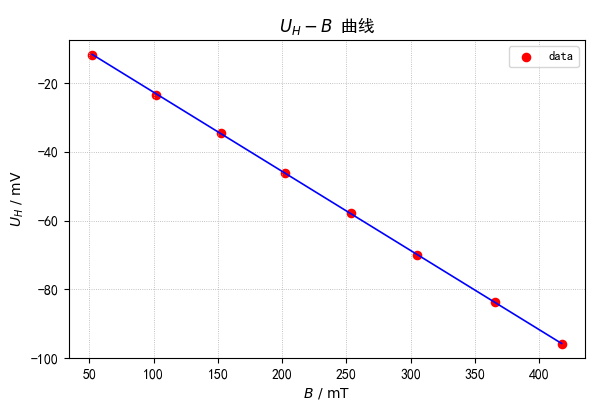
\includegraphics[width=0.8\textwidth]{Figure_4.png}
    \caption{}
\end{figure}
曲线斜率 $K'=-0.23018$，霍尔元件灵敏度 $K=K'I_H=-0.23018\ \mathrm{mV/(mT\cdot mA)}$，为 N 型霍尔元件。

\section{总结}
这次实验让我受益匪浅。通过亲手测量螺线管轴向磁场的分布情况，我不仅深入理解了
霍尔效应各种副效应的原理，还掌握了利用电流换向法准确获取数据的实验技巧。处理数据
时，由 $U_1'$ 和 $U_2'$ 计算出的 $B-X$ 曲线从边缘陡增到中心平稳、再到另一端下降的对称过
程，直观地让我看到了通电螺线管内部磁场的均匀性分布特点，并验证了有限长螺线管磁场
的理论模型。这次实验不仅锻炼了我的动手实践能力和数据处理分析能力，更让我体会到了
物理规律从理论推导到实验验证的严谨，培养了我在科学实验中耐心细致、客观求实的态度。
\end{document}